\documentclass[tikz,border=5pt]{standalone}
\usetikzlibrary{arrows.meta,positioning}
\begin{document}
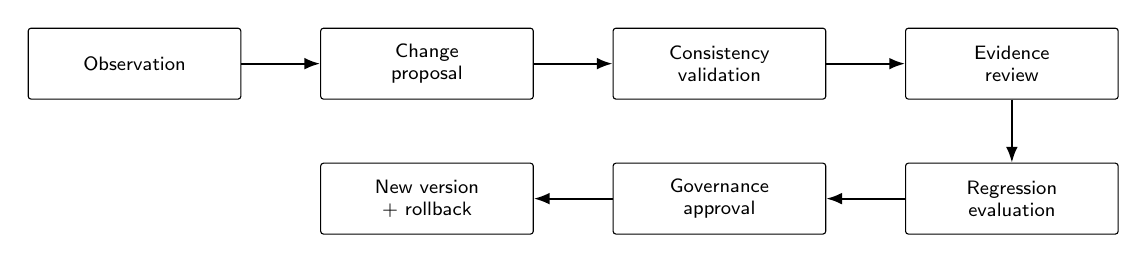
\begin{tikzpicture}[
  box/.style={draw, rounded corners=1pt, minimum width=27mm, minimum height=9mm, align=center, font=\sffamily\scriptsize},
  arrow/.style={-{Latex[length=2mm]}, thick}
]
\node[box] (obs) {Observation};
\node[box, right=of obs] (prop) {Change\\proposal};
\node[box, right=of prop] (valid) {Consistency\\validation};
\node[box, right=of valid] (review) {Evidence\\review};
\node[box, below=8mm of review] (regress) {Regression\\evaluation};
\node[box, left=of regress] (gov) {Governance\\approval};
\node[box, left=of gov] (version) {New version\\+ rollback};
\draw[arrow] (obs) -- (prop);
\draw[arrow] (prop) -- (valid);
\draw[arrow] (valid) -- (review);
\draw[arrow] (review) -- (regress);
\draw[arrow] (regress) -- (gov);
\draw[arrow] (gov) -- (version);
\end{tikzpicture}
\end{document}
